\documentclass{standalone}
\usepackage{tikz}
\usetikzlibrary{patterns, positioning}


\begin{document}
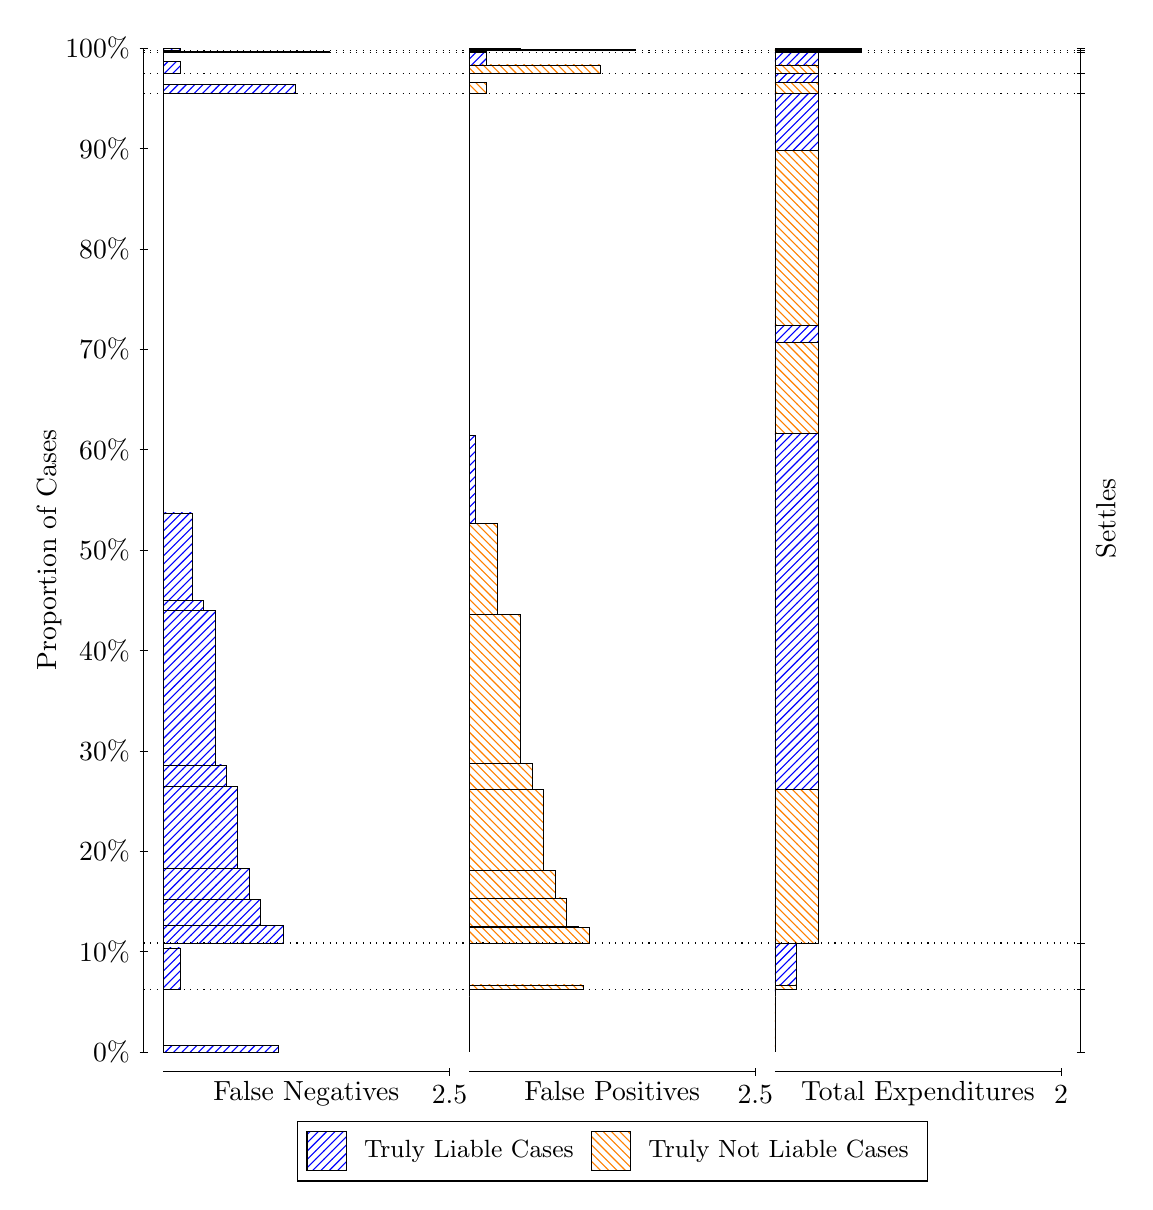
\begin{tikzpicture}
\draw[black, very thin] (1.5,1.75) -- (1.5,14.5);
\node[rotate=90, text=black, anchor=center] at (0.3, 8.125) {Proportion of Cases};
\draw[black, very thin] (1.45,1.75) -- (1.55,1.75);
\node[text=black, anchor=east] at (1.45, 1.75) {0\%};
\draw[black, very thin] (1.45,3.025) -- (1.55,3.025);
\node[text=black, anchor=east] at (1.45, 3.025) {10\%};
\draw[black, very thin] (1.45,4.3) -- (1.55,4.3);
\node[text=black, anchor=east] at (1.45, 4.3) {20\%};
\draw[black, very thin] (1.45,5.575) -- (1.55,5.575);
\node[text=black, anchor=east] at (1.45, 5.575) {30\%};
\draw[black, very thin] (1.45,6.85) -- (1.55,6.85);
\node[text=black, anchor=east] at (1.45, 6.85) {40\%};
\draw[black, very thin] (1.45,8.125) -- (1.55,8.125);
\node[text=black, anchor=east] at (1.45, 8.125) {50\%};
\draw[black, very thin] (1.45,9.4) -- (1.55,9.4);
\node[text=black, anchor=east] at (1.45, 9.4) {60\%};
\draw[black, very thin] (1.45,10.675) -- (1.55,10.675);
\node[text=black, anchor=east] at (1.45, 10.675) {70\%};
\draw[black, very thin] (1.45,11.95) -- (1.55,11.95);
\node[text=black, anchor=east] at (1.45, 11.95) {80\%};
\draw[black, very thin] (1.45,13.225) -- (1.55,13.225);
\node[text=black, anchor=east] at (1.45, 13.225) {90\%};
\draw[black, very thin] (1.45,14.5) -- (1.55,14.5);
\node[text=black, anchor=east] at (1.45, 14.5) {100\%};

\draw[black, very thin] (13.4,1.75) -- (13.4,14.5);
\draw[black, very thin] (13.35,1.75) -- (13.45,1.75);
\node[anchor=west] at (13.35, 1.75) {};
\draw[black, very thin] (13.35,2.5408) -- (13.45,2.5408);
\node[anchor=west] at (13.35, 2.5408) {};
\draw[black, very thin] (13.35,3.1339) -- (13.45,3.1339);
\node[anchor=west] at (13.35, 3.1339) {};
\draw[black, very thin] (13.35,13.924) -- (13.45,13.924);
\node[anchor=west] at (13.35, 13.924) {};
\draw[black, very thin] (13.35,14.174) -- (13.45,14.174);
\node[anchor=west] at (13.35, 14.174) {};
\draw[black, very thin] (13.35,14.444) -- (13.45,14.444);
\node[anchor=west] at (13.35, 14.444) {};
\draw[black, very thin] (13.35,14.472) -- (13.45,14.472);
\node[anchor=west] at (13.35, 14.472) {};
\draw[black, very thin] (13.35,14.5) -- (13.45,14.5);
\node[anchor=west] at (13.35, 14.5) {};

\draw[black, very thin, pattern color=blue, pattern=north east lines] (1.75,1.75) rectangle (3.2033,1.8332);
\draw[black, very thin, pattern color=orange, pattern=north west lines] (1.75,1.8332) rectangle (1.75,2.5408);
\draw[black, very thin, pattern color=blue, pattern=north east lines] (1.75,2.5408) rectangle (1.968,3.0715);
\draw[black, very thin, pattern color=orange, pattern=north west lines] (1.75,3.0715) rectangle (1.75,3.1339);
\draw[black, very thin, pattern color=blue, pattern=north east lines] (1.75,3.1339) rectangle (3.276,3.3567);
\draw[black, very thin, pattern color=blue, pattern=north east lines] (1.75,3.3567) rectangle (2.9853,3.689);
\draw[black, very thin, pattern color=blue, pattern=north east lines] (1.75,3.689) rectangle (2.84,4.0779);
\draw[black, very thin, pattern color=blue, pattern=north east lines] (1.75,4.0779) rectangle (2.6947,5.1257);
\draw[black, very thin, pattern color=blue, pattern=north east lines] (1.75,5.1257) rectangle (2.5493,5.3974);
\draw[black, very thin, pattern color=blue, pattern=north east lines] (1.75,5.3974) rectangle (2.404,7.355);
\draw[black, very thin, pattern color=blue, pattern=north east lines] (1.75,7.355) rectangle (2.2587,7.4807);
\draw[black, very thin, pattern color=blue, pattern=north east lines] (1.75,7.4807) rectangle (2.1133,8.5977);
\draw[black, very thin, pattern color=orange, pattern=north west lines] (1.75,8.5977) rectangle (1.75,13.924);
\draw[black, very thin, pattern color=blue, pattern=north east lines] (1.75,13.924) rectangle (3.4213,14.035);
\draw[black, very thin, pattern color=orange, pattern=north west lines] (1.75,14.035) rectangle (1.75,14.174);
\draw[black, very thin, pattern color=blue, pattern=north east lines] (1.75,14.174) rectangle (1.968,14.333);
\draw[black, very thin, pattern color=orange, pattern=north west lines] (1.75,14.333) rectangle (1.75,14.444);
\draw[black, very thin, pattern color=blue, pattern=north east lines] (1.75,14.444) rectangle (3.8573,14.453);
\draw[black, very thin, pattern color=orange, pattern=north west lines] (1.75,14.453) rectangle (1.75,14.472);
\draw[black, very thin, pattern color=blue, pattern=north east lines] (1.75,14.472) rectangle (1.968,14.491);
\draw[black, very thin, pattern color=orange, pattern=north west lines] (1.75,14.491) rectangle (1.75,14.5);
\draw[black, very thin, pattern color=orange, pattern=north west lines] (5.6333,1.75) rectangle (5.6333,2.4576);
\draw[black, very thin, pattern color=blue, pattern=north east lines] (5.6333,2.4576) rectangle (5.6333,2.5408);
\draw[black, very thin, pattern color=orange, pattern=north west lines] (5.6333,2.5408) rectangle (7.0867,2.6032);
\draw[black, very thin, pattern color=blue, pattern=north east lines] (5.6333,2.6032) rectangle (5.6333,3.1339);
\draw[black, very thin, pattern color=orange, pattern=north west lines] (5.6333,3.1339) rectangle (7.1593,3.3287);
\draw[black, very thin, pattern color=orange, pattern=north west lines] (5.6333,3.3287) rectangle (7.014,3.3486);
\draw[black, very thin, pattern color=orange, pattern=north west lines] (5.6333,3.3486) rectangle (6.8687,3.7066);
\draw[black, very thin, pattern color=orange, pattern=north west lines] (5.6333,3.7066) rectangle (6.7233,4.0513);
\draw[black, very thin, pattern color=orange, pattern=north west lines] (5.6333,4.0513) rectangle (6.578,5.0839);
\draw[black, very thin, pattern color=orange, pattern=north west lines] (5.6333,5.0839) rectangle (6.4327,5.4183);
\draw[black, very thin, pattern color=orange, pattern=north west lines] (5.6333,5.4183) rectangle (6.2873,7.3054);
\draw[black, very thin, pattern color=orange, pattern=north west lines] (5.6333,7.3054) rectangle (5.9967,8.4606);
\draw[black, very thin, pattern color=blue, pattern=north east lines] (5.6333,8.4606) rectangle (5.706,9.5776);
\draw[black, very thin, pattern color=blue, pattern=north east lines] (5.6333,9.5776) rectangle (5.6333,13.924);
\draw[black, very thin, pattern color=orange, pattern=north west lines] (5.6333,13.924) rectangle (5.8513,14.064);
\draw[black, very thin, pattern color=blue, pattern=north east lines] (5.6333,14.064) rectangle (5.6333,14.174);
\draw[black, very thin, pattern color=orange, pattern=north west lines] (5.6333,14.174) rectangle (7.3047,14.285);
\draw[black, very thin, pattern color=blue, pattern=north east lines] (5.6333,14.285) rectangle (5.8513,14.444);
\draw[black, very thin, pattern color=orange, pattern=north west lines] (5.6333,14.444) rectangle (5.8513,14.463);
\draw[black, very thin, pattern color=blue, pattern=north east lines] (5.6333,14.463) rectangle (5.6333,14.472);
\draw[black, very thin, pattern color=orange, pattern=north west lines] (5.6333,14.472) rectangle (7.7407,14.481);
\draw[black, very thin, pattern color=blue, pattern=north east lines] (5.6333,14.481) rectangle (6.2873,14.5);
\draw[black, very thin, pattern color=orange, pattern=north west lines] (9.5167,1.75) rectangle (9.5167,2.4576);
\draw[black, very thin, pattern color=blue, pattern=north east lines] (9.5167,2.4576) rectangle (9.5167,2.5408);
\draw[black, very thin, pattern color=orange, pattern=north west lines] (9.5167,2.5408) rectangle (9.7892,2.6032);
\draw[black, very thin, pattern color=blue, pattern=north east lines] (9.5167,2.6032) rectangle (9.7892,3.1339);
\draw[black, very thin, pattern color=orange, pattern=north west lines] (9.5167,3.1339) rectangle (10.062,5.0839);
\draw[black, very thin, pattern color=blue, pattern=north east lines] (9.5167,5.0839) rectangle (10.062,9.6038);
\draw[black, very thin, pattern color=orange, pattern=north west lines] (9.5167,9.6038) rectangle (10.062,10.759);
\draw[black, very thin, pattern color=blue, pattern=north east lines] (9.5167,10.759) rectangle (10.062,10.982);
\draw[black, very thin, pattern color=orange, pattern=north west lines] (9.5167,10.982) rectangle (10.062,13.203);
\draw[black, very thin, pattern color=blue, pattern=north east lines] (9.5167,13.203) rectangle (10.062,13.924);
\draw[black, very thin, pattern color=orange, pattern=north west lines] (9.5167,13.924) rectangle (10.062,14.064);
\draw[black, very thin, pattern color=blue, pattern=north east lines] (9.5167,14.064) rectangle (10.062,14.174);
\draw[black, very thin, pattern color=orange, pattern=north west lines] (9.5167,14.174) rectangle (10.062,14.285);
\draw[black, very thin, pattern color=blue, pattern=north east lines] (9.5167,14.285) rectangle (10.062,14.444);
\draw[black, very thin, pattern color=orange, pattern=north west lines] (9.5167,14.444) rectangle (10.607,14.463);
\draw[black, very thin, pattern color=blue, pattern=north east lines] (9.5167,14.463) rectangle (10.607,14.472);
\draw[black, very thin, pattern color=orange, pattern=north west lines] (9.5167,14.472) rectangle (10.607,14.481);
\draw[black, very thin, pattern color=blue, pattern=north east lines] (9.5167,14.481) rectangle (10.607,14.5);
\draw[black, dotted] (1.5,2.5408) -- (13.4,2.5408);
\draw[black, dotted] (1.5,3.1339) -- (13.4,3.1339);
\draw[black, dotted] (1.5,13.924) -- (13.4,13.924);
\draw[black, dotted] (1.5,14.174) -- (13.4,14.174);
\draw[black, dotted] (1.5,14.444) -- (13.4,14.444);
\draw[black, dotted] (1.5,14.472) -- (13.4,14.472);
\draw[black, very thin] (1.75,1.5) -- (5.3833,1.5);
\node[text=black, anchor=north] at (3.5667, 1.5) {False Negatives};
\draw[black, very thin] (5.3833,1.45) -- (5.3833,1.55);
\node[text=black, anchor=north] at (5.3833, 1.45) {2.5};

\draw[black, very thin] (5.6333,1.5) -- (9.2667,1.5);
\node[text=black, anchor=north] at (7.45, 1.5) {False Positives};
\draw[black, very thin] (9.2667,1.45) -- (9.2667,1.55);
\node[text=black, anchor=north] at (9.2667, 1.45) {2.5};

\draw[black, very thin] (9.5167,1.5) -- (13.15,1.5);
\node[text=black, anchor=north] at (11.333, 1.5) {Total Expenditures};
\draw[black, very thin] (13.15,1.45) -- (13.15,1.55);
\node[text=black, anchor=north] at (13.15, 1.45) {2};



\node[text=black, centered, rotate=90] at (13.72, 8.5292) {Settles};





\draw (7.449999999999999,1.5) node[draw=none] (baseCoordinate) {};
\begin{scope}[align=center]
        \matrix[scale=0.5, draw=black, below=0.5cm of baseCoordinate, nodes={draw}, column sep=0.1cm]{
            \node[rectangle, draw, minimum width=0.5cm, minimum height=0.5cm, pattern color=blue, pattern=north east lines] {}; &
            \node[draw=none, font=\small, text=black] (B) {Truly Liable Cases}; &
            \node[rectangle, draw, minimum width=0.5cm, minimum height=0.5cm, pattern color=orange, pattern=north west lines] {}; &
            \node[draw=none, font=\small, text=black] (B) {Truly Not Liable Cases}; \\
            };
\end{scope}

\end{tikzpicture}
\end{document}